\chapter{Machine Learning}
\label{ch:ml}
Machine learning is a branch of mathematics and computer science that attempts to build models that can learn from data and/or generalise to unseen data to perform a task without explicit instructions, and the specific term dates back to 1959~\cite{samuel1959some}. 

While many other models have been proposed, it's not necessary to exhaustively enumerate them here. 
For a comprehensive study of the matter, see ``Understanding Machine Learning''~\cite{shalev2014understanding}. 
However, a subset of models is outlined below to now only introduce the models used throughout the text, but to develop an intuition about the various considerations of an ML model and the resultant limitations. 
Figure~\ref{fig:data_model_comparison} provides a visualisation of the models discussed below and their efficacy on different types of data. 



% \cm{TODO: define features, samples, model, over/under-determined, x, y, labels/targets, decision boundary. hard labels soft labels}


\begin{figure}[p]
    \centering
    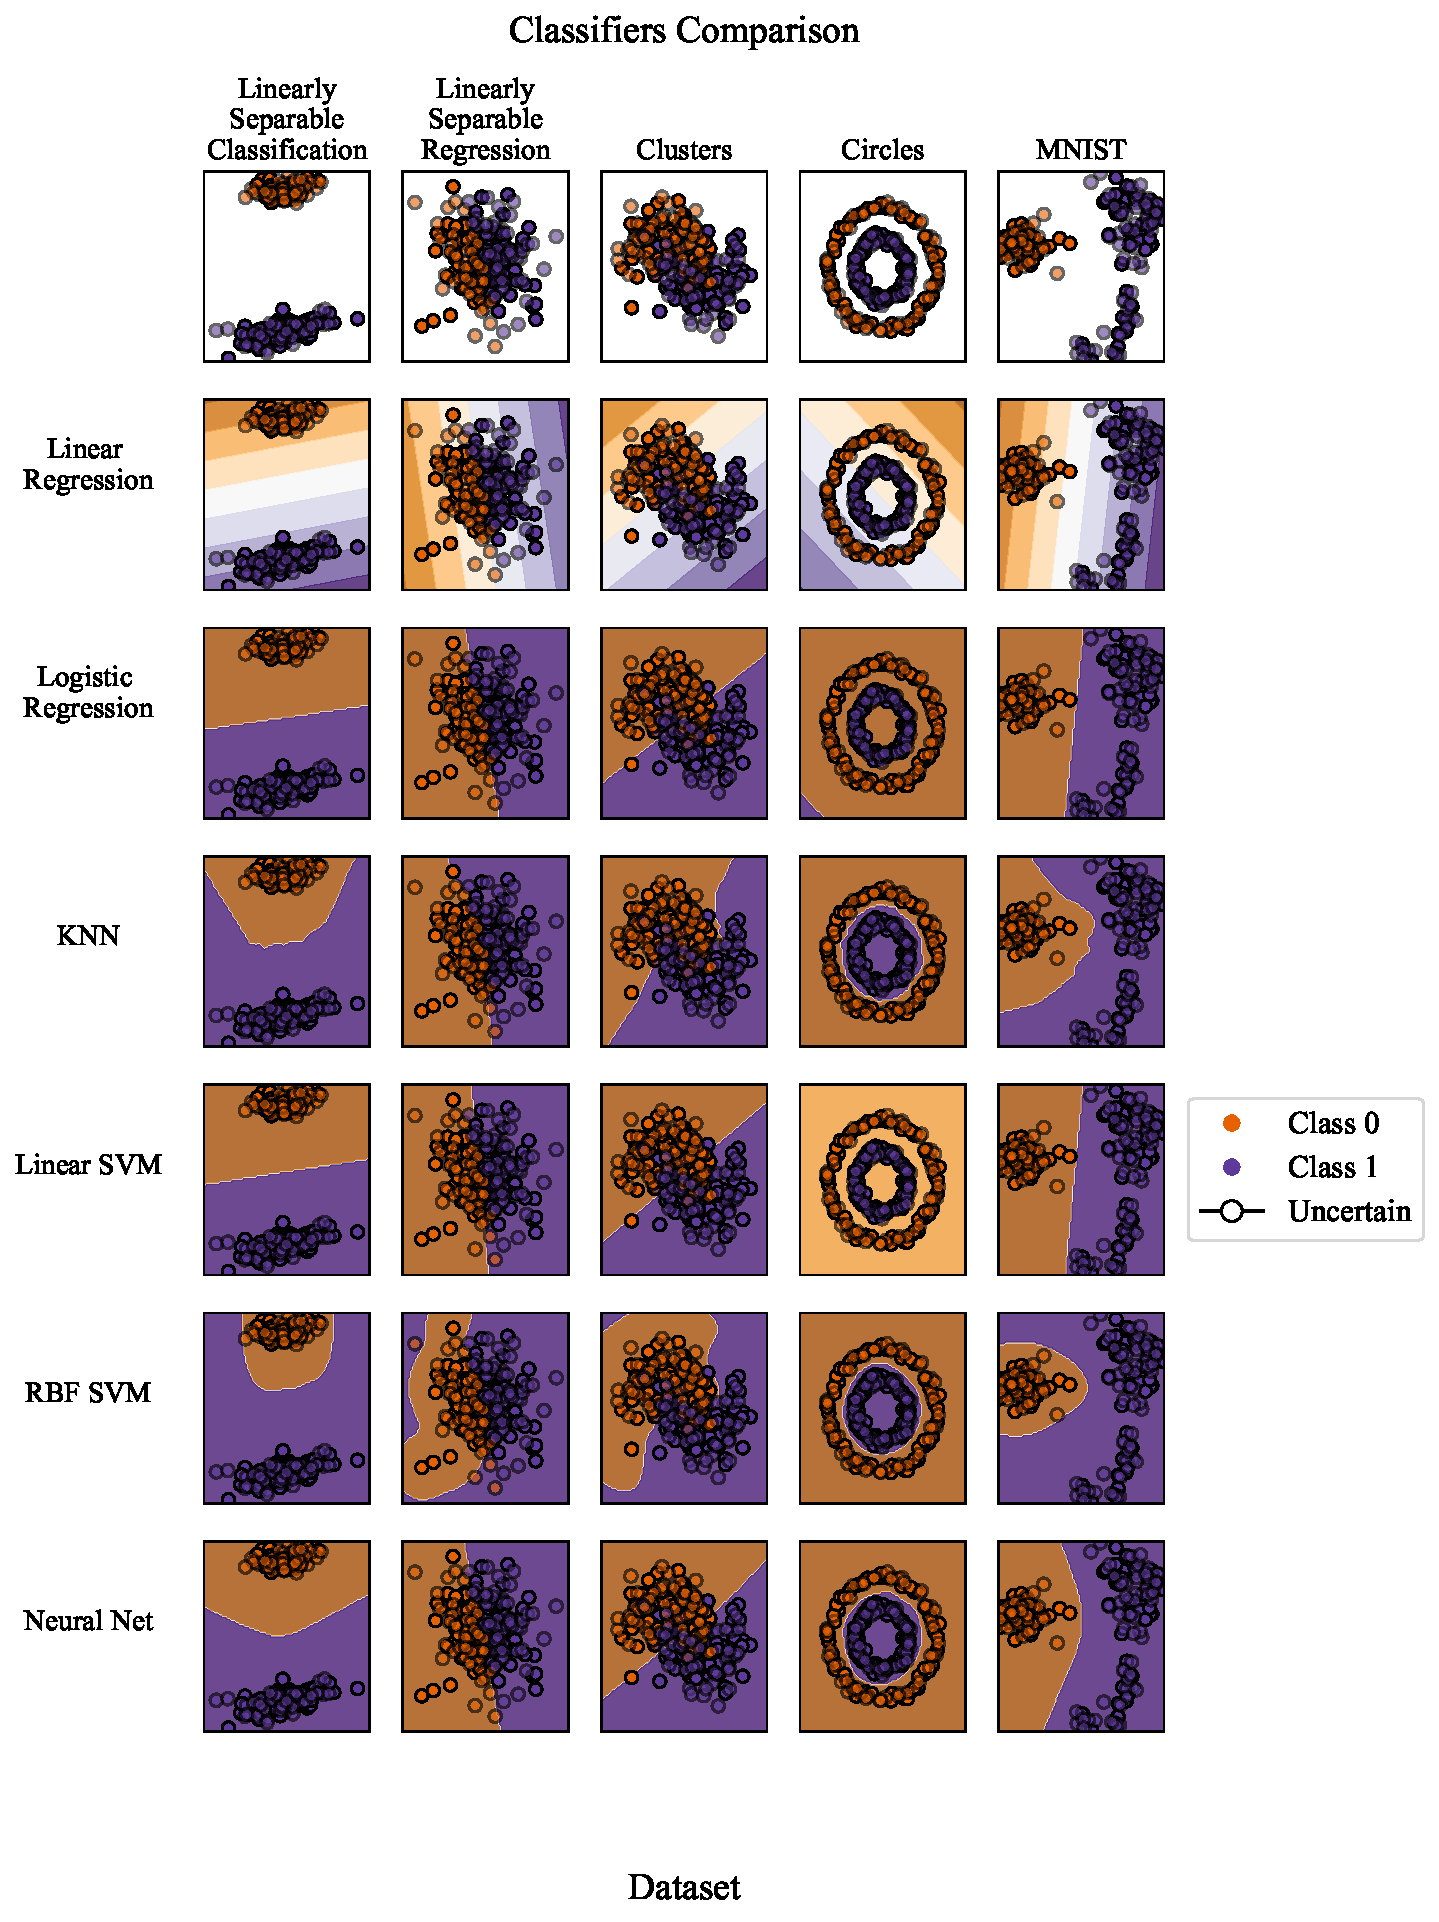
\includegraphics[width=.7\textheight, angle=90]{images/dataset_model_comparison.pdf}
    \caption{
    Each row depicts a different dataset where the values are classified into one of two classes, depicted by red or blue dots. 
    The model's \textit{decision boundary} is depicted using the red and blue gradients with darker colours corresponding to a more confident decision. 
    The first column depicts the raw input data and the true labels.
    Each other columns depicts the prediction using colour.
    The first 4 rows used generated two-dimensional data and the last row depicts a two-dimensional projection of the MNIST image dataset discussed in Section~\ref{subsec:methods-data} (since it would be impossible to plot the data in the 64 dimensions MNIST provides in the form of black and white pixels).
    }
    \label{fig:data_model_comparison}
    % \cm{todo: swap rows/columns, make full page, and update the caption accordingly}
\end{figure}


\section{Classical Methods}
Classical machine learning methods refer to models that rely on established statistical principles and typically make assumptions about the data structure. 
These models are often interpretable, computationally efficient, and serve as strong baselines for more complex approaches. 
Some of the most well-known classical methods include linear models, logistic regression, support vector classifiers (SVCs), and clustering algorithms like k-nearest neighbours (KNN).

\subsection{Parametric Models}
Parametric models are a class of models that summarize the data through a set of fixed parameters. 
These models assume a specific form for the underlying distribution of the data and require learning a finite number of parameters from the data. 
Once the parameters are estimated during model training, the model is fully defined, and predictions can be made.

\subsubsection{Linear Regression}
Linear regression is one of the simplest and most widely used models for supervised learning tasks. 
It models the relationship between a scalar dependent variable and one or more independent variables by fitting a linear equation to the observed data. 
However, there are certain disadvantages to this approach. 
Linear regression assumes that the relationship between the features and the target variable is, in fact, linear, which does not hold in many real-world scenarios.
See Figure~\ref{fig:data_model_comparison} to visualise the types of data that can be classified by this model.
Additionally, if the independent variables  are highly correlated, it may lead to multicollinearity, which can cause instability in the estimated parameters.
Despite its limitations, linear regression serves as a foundational model in machine learning, providing a solid basis for understanding more complex techniques.


\subsubsection{Logistic Regression}
Logistic regression is a widely used classification algorithm for binary outcomes, modelling the probability that a given input belongs to a particular class. 
Unlike linear regression, logistic regression uses a sigmoid (logistic) function to constrain the output between 0 and 1, making it ideal for probability estimation. 
Rather than producing an output that corresponds to a value in the range of  $(-\infty, +\infty)$ (as in the case of linear regression), it produces an output in the range $(0,1)$ which corresponds nicely with the notion of probability. 
In short, a logistic regression model produces an output that answers the question: ``what is the probability of an event when we assume a linear relationship between the input and the model weights?''


\subsubsection{Normality}

Throughout this thesis, data \textit{normalisation} is employed to standardise the columns of input data and assumes that the mean and standard deviation can be calculated from a sample of the true population.
Normalisation involves subtracting the mean from each sample and dividing by the standard deviation, resulting in values that represent the number of standard deviations each point lies from the mean. 
This transformation ensures comparability across features, even when their original scales differ significantly.

A key motivation for normalisation is to improve the numerical \textit{stability} of machine learning models. 
Normalised inputs reduce the risk of large output fluctuations in response to small input changes, thereby facilitating robustness.
The effectiveness of this process relies on the assumption that data is independently and identically distributed (i.i.d.). 
\textit{Independence} means that one observation does not influence another, while \textit{identically distributed} implies all samples originate from the same underlying distribution. 
These assumptions are foundational to many statistical methods.

Moreover, the Central Limit Theorem (CLT) supports the use of normalisation and normality-based techniques. 
It states that, for a sufficiently large sample size, the distribution of the sample mean approximates a normal distribution regardless of the original data distribution~\cite{stats}. 
In machine learning, this justifies the use of batch-wise statistics during training, as batch means tend to be normally distributed, enabling the application of methods that assume or benefit from normality~\cite{shalev2014understanding}.



\subsection{Non-Parametric Models}
Non-parametric models are a category of statistical models that do not assume a fixed number of parameters. 
Instead, they allow for greater flexibility in modelling complex datasets by letting the model structure grow with the data. 
This adaptability makes them particularly useful in situations where the underlying data distribution is unknown or highly variable. 
These models have no fixed assumptions about the underlying distribution of the data and some popular choices are outlined below. 

\subsubsection{KNN}
One non-parametric model used is $k$-nearest neighbours (k-NN), which is a type of instance-based learning where a data point is classified based on the majority class of its $k$ closest neighbours according to some relevant notion of distance. 
This model is widely used for classification tasks, and in Paper 5, it is specifically employed to cluster spam and non-spam internet traffic and content.

\subsubsection{Bootstrapping}

Another non-parametric model, called bootstrapping, is particularly useful for assessing the uncertainty or variability of an estimator without relying on strong parametric assumptions about the data's distribution. 
This method is used throughout the thesis to generate plots from the measured data, providing the uncertainty estimations that are denoted with error bars. 

\subsubsection{SVM}
Support Vector Machines (SVM) are a powerful class of supervised learning models used for classification and regression tasks. 
The core idea of SVM is to find a surface (often called a \textit{hyper-plane}) that best separates data points of different classes in a high-dimensional space.
While the basic SVM can be considered a parametric model (as it assumes that the data can be separated by a line), it becomes non-parametric when using kernel functions, which allow it to capture complex relationships in the data. 
This latter version is used in Papers II and V. 

These kernelised models are examined in greater detail in Papers II and  V. 
SVMs are effective when the number of features is much larger than the number of samples, which is common in text classification or biological data. 
This is also likely in the case of high resolution images as each megapixel of resolution yields 1 feature for each colour channel on each pixel-- meaning that 1 megapixel red/green/blue images correspond to 3 million features.

The use of kernel functions allows SVMs to perform well even when the data is not linearly separable by transforming the input into a higher-dimensional space.
Through kernel functions, SVMs can create complex, non-linear decision boundaries. 
Training an SVM can be slow, especially with large datasets, since it requires solving a quadratic programming problem~\cite{bottou2007support}.
The run-time of SVMs does not scale well with large datasets, both in terms of training time and memory requirements~\cite{bottou2007support}.
The decision boundary generated by SVMs, particularly with non-linear kernels, can be difficult to interpret~\cite{shalev2014understanding}.




\section{Neural Networks}
Neural networks are another class of ML models that can be both parametric~\cite{parametric_neural_network} and non-parametric~\cite{non_parametric_neural_network}. 
A neural network can be thought of as a graph composes of nodes that are connected by edges, composed of an input layer, one or more ``hidden'' layers that perform complex (non-linear) operations on the input data, and an output layer that returns a number, a vector of probabilities (called a \textit{soft label}), or a series of binary classifications (called a \textit{hard label}). 
Figure~\ref{fig:neural_network} depicts a simple neural network using circles to represent nodes, black lines to represent edges, and colour is used to identify input, hidden, and output layers. 

\begin{figure}[!ht]
\centering
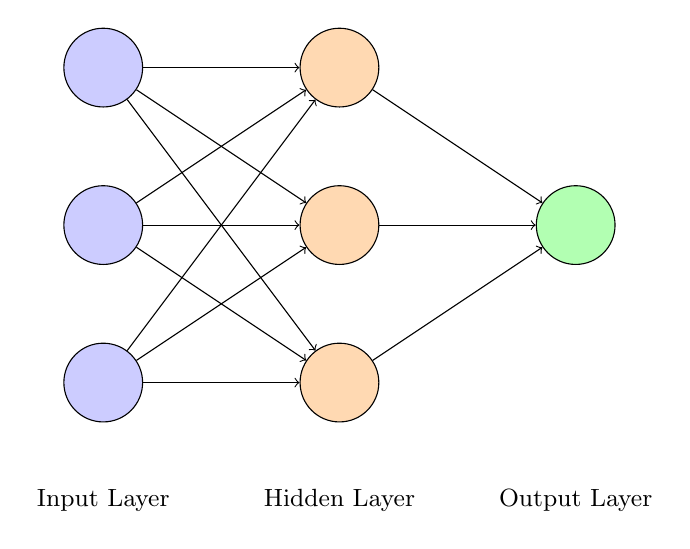
\begin{tikzpicture}[
    neuron/.style={circle, draw, minimum size=1cm},
    input neuron/.style={neuron, fill=blue!20},
    hidden neuron/.style={neuron, fill=orange!30},
    output neuron/.style={neuron, fill=green!30},
    layer/.style={draw=none, align=center},
    every node/.style={font=\small}
  ]

  % Input Layer
  \node[input neuron] (I-1) at (0,2) {};
  \node[input neuron] (I-2) at (0,0) {};
  \node[input neuron] (I-3) at (0,-2) {};
  \node[layer] at (0,-3.5) {Input Layer};

  % Hidden Layer
  \node[hidden neuron] (H-1) at (3,2) {};
  \node[hidden neuron] (H-2) at (3,0) {};
  \node[hidden neuron] (H-3) at (3,-2) {};
  \node[layer] at (3,-3.5) {Hidden Layer};

  % Output Layer
  \node[output neuron] (O-1) at (6,0) {};
  \node[layer] at (6,-3.5) {Output Layer};

  % Connections
  \foreach \i in {1,2,3}
    \foreach \h in {1,2,3}
      \draw[->] (I-\i) -- (H-\h);

  \foreach \h in {1,2,3}
    \draw[->] (H-\h) -- (O-1);

\end{tikzpicture}
\caption{A simple neural network with three layers. The input (blue), hidden (orange), and output (green) layers are colour-coded for clarity. The arrows indicate the flow of data.}
\label{fig:neural_network}
\end{figure}

Typically, state-of-the-art models are significantly more complex than the one pictured in Figure~\ref{fig:neural_network} and often rely on large numbers of hidden layers, complex structures (also called \textit{architectures}) that, for example, provide mechanisms to reinforce a certain behvaiour~\cite{reinforcement_learning} or enable time-dependent model configuration~\cite{lstm}.
Model architectures are sometimes chosen in an effort to model a particular biological~\cite{biomimicry_nn} or physical process~\cite{physics_nn}, though model architectures are often determined by brute-force trial and error~\cite{nn_architectures_brute_force}.

Regardless of the model architecture, training a neural network requires the definition of a loss function—a quantitative measure of how far the model’s output deviates from the expected result. 
The choice of loss function is often dictated by the task at hand: for example, cross-entropy loss is widely used for classification problems~\cite{shalev2014understanding} because it naturally penalizes confident but incorrect predictions; whereas mean squared error~(MSE)~\cite{stats} is commonly applied in regression tasks where the goal is to minimize the average squared difference between predicted and actual values. 
More sophisticated loss functions can encode domain-specific requirements, such as robustness to outliers~\cite{zhang2015outlier}, uncertainty visualisation~\cite{model_uncertainty}, or fairness constraints~\cite{mehrabi2021survey}, and can be custom-designed to reflect complex trade-offs or safety margins.

The optimization process involves adjusting the network’s internal parameters—typically millions or even billions of weights and biases—to minimize the chosen loss function across a given dataset. 
This is most often done using stochastic gradient descent (SGD) or one of its many variants (e.g., Adam~\cite{adam}, RMSProp~\cite{rmsprop}, or Adadelta~\cite{adadelta}) which iteratively updates model parameters in the direction that minimises the chosen loss function by comparing model predictions to the ground truth.

The optimization landscape of a deep neural network is highly non-convex--- it often contains numerous local minima, saddle points, and flat regions. 
In practice, modern optimization algorithms, combined with techniques like learning rate scheduling~\cite{learning_rate_scheduling}, regularization~\cite{xu2009robustness,jakubovitz2018improving,ross2018improving}, momentum~\cite{momentum}, and batch normalization~\cite{batch_normalisation}, enable effective navigation of this complex terrain. 
However, convergence to a low loss value does not necessarily imply generalisation to new data.
As a result, the optimization process is closely tied to  the choice in validation metric~\cite{carlini2019evaluating} and techniques for measuring generalisation error like cross-validation scoring~\cite{shalev2014understanding} are used to ensure that the network not only performs well on training data but also works well \textit{in general}.

Furthermore, in domains such as healthcare, aviation, or autonomous systems, loss functions and optimization criteria may be carefully designed to reflect asymmetric costs of error~\cite{meyers2023safety}. 
For instance, this might mean penalizing false negatives more heavily than false positives when a missed detection could result in harm than a false positive. 
In other cases, this might mean providing mechanisms to notifying a user when a given classification is uncertain~\cite{model_uncertainty}.
This further reinforces the idea that model training is not merely a numerical process, but a design decision that must align with the broader goals of safety, reliability, and ethical deployment.
Nevertheless, even an excellent score on well chosen metric does not guarantee legally compliant performance in the presence of an adversary~\cite{meyers2023safety,meyers2024massively,trashfire,meyers_aft}, which are characterised further in Chapter 4. 
For now, suffice it to say that not only do the regulatory concerns outlined in Chapter 2 remain persistent threats to large-scale machine learning methods, but that they raise serious ethical concerns more broadly.

\section{The Ethics of ML}
\label{sec:ethics}
The problems with the typical approach to ML are numerous. 
Recently, marginal gains in accuracy have relied on increasingly larger models to produce marginal gains~\cite{desislavov2021compute}. 
These models rely on massive datasets~\cite{desislavov2021compute,vapnik1994measuring,blumer1989learnability}, from an ever-shrinking number of sources~\cite{koch2021reduced}, leading to gender-biased models~\cite{lu2020gender}, race-biased models~\cite{buolamwini2018gender}, and critical design errors~\cite{banks2018driver}. 
This trend isn't new and goes back decades~\cite{corsaro1982something,ramirez2000resource,buolamwini2018gender}. 
Despite this, it has been suggested that large scale ML methods be used to detect (\textit{potentially}) illegal material~\cite{abelson2021bugs}.
Since client-side monitoring with neural networks was recently the subject of a proposal by the EU parliament to stop the spread of offensive and harmful online contact, it can be used as a simple case study in how \textit{obviously} ``good'' models have inherent risks.
One, these models are not nearly reliable enough to be deployed in situations that can negatively effect a human, which is detailed in the previous chapter. 
Second, these models can reveal the private data used to train the model~\cite{extraction_attack} or used to generate novel content that is similar to restricted images~\cite{deepface_attack}.
Third, these models are inherently biased--- relying on statistical assumptions that harm already marginalised groups \cite{buolamwini2018gender}. 
Fourth, the existence of the model comes with unforeseen environmental and societal costs-- potentially chilling dissent or speech~\cite{abelson2021bugs}, using immense computational resources~\cite{ai_power}, and outsourcing of the data labelling to low wage workers who have to view the offensive content~\cite{ai_inequity}.
Finally, modern ML systems in general have questionable reliability on edge cases, but nevertheless induce real experts to misjudge the quality of the model output~\cite{chatgptlawyer,teslasleep1,teslasleep2,teslasleep3,perry2023users,rosenbacke2024ai}.
In short, there are many ethical questions to consider when deploying an ML model which have been clustered into efficacy, privacy, security, reliability, and the environment.  
In the following,  




\subsection{Reliability}
\label{subsec:reliability}
Fundamentally, ML systems are just statistical models that have the the ability to over-generalise.
ML models have shown themselves capable of performing exceptionally well on a wide variety of tasks. 
For example, there are thousands of papers that report
However, much research has also noted the fragility of these models to small changes in the input space. 
One particular concerning example is the inability of state-of-the-art image classification systems to handle data that comes from a different distribution than the training set~\cite{bungert2023understanding}. 
One proposed source of this error is ``hidden stratification''--- the unknown subsets of the data that are unaccounted for in the model~\cite{hidden_stratification}.
Another often-discussed source of unreliability is the ``long-tail problem'' that describes the problem of the wide distribution of real-world cases outside of the ``normal'' distribution learned from the training set.
This 2021 survey of wildlife identification models examined methods for mitigating the effect of these out-of-distribution new samples and their best attempt still confidently returned an incorrect answer nearly 30\% of the time.
Another author notes that the standard model output layers do not even return meaningful confidence intervals~\cite{medical_failure_detection}.
Some authors \cite{birhane2021algorithmic} recommend a set of ethics that centres machine learning research on groups mostly likely to be adversely effected. 
However, since these groups tend to be marginalised or statistical outliers compared to dominant groups, there's an inherent tension within this recommendation. 
Let's take the case of the autonomous (self-driving) car. On one hand, we would like cars to not mistake women, minority groups, or gender non-conforming people for inanimate objects. 
On the other hand, the statistical variance introduced by these statistically less ``normal'' subsets of people will cause a degradation of performance for the ``average'' user. 
Is it more fair to reduce the accuracy overall for the sake of statistically ``abnormal'' groups rather than maximise the performance on the statistically average person? 
This tension was proven to be inherent to the statistical methods underlying machine learning systems \cite{carlini_towards_2017}. 
This tension is widely discussed in the literature on fairness for machine learning as well~\cite{feuerriegel2020fair,van2021fairness,corbett2018measure}. 
To be clear, this isn't a problem that is restricted to discrete classes like skin colour or apparent gender, but is can be extended to any statistically ``abnormal'' situation.
While some mitigation strategies have been proposed~\cite{medical_failure_detection,medical_ML_methodology}
The intention here is not to single-out medical imaging as a potentially risky application of ML as industrial control~\cite{ai_industry} software, aviation control software~\cite{ai_aviation}, autonomous cars~\cite{ai_automotive}, bank loaning algorithms~\cite{ai_finance}, criminal justice administration tools~\cite{ai_prison}, predictive policing algorithms~\cite{ai_security}, home pricing algorithms~\cite{ai_home_pricing}, and computer-vision based security checkpoints~\cite{ai_luggage} are built from the same models.


\subsubsection{Reproducibility}
\label{subsec:reproducibility}

Unlike the experiments detailed in the included papers, ML research models are typically not reproducible. 
Firstly, there is a problem of scale as ML research has increasingly shifted to industry due to the massive costs associated with training state-of-the-art models~\cite{ai_cost_comparison}. 
This is in no small part due to the scale of both modern models and their associated datasets~\cite{desislavov2021compute,ai_power} which have grown in size~\cite{desislavov2021compute} and increasingly come from fewer sources~\cite{koch2021reduced}. 
For example, commercially deployed image recognition systems~and large-language models can cost millions of dollars of compute time to train~\cite{ai_cost_comparison}, making reproducing state-of-the-art research infeasible under the current peer review system. 
Even when model architectures are fully released, critical components can be omitted or under-specified---including details about training schedules, hyper-parameter selection, hardware or network configuration, and random seed initialisation~\cite{medical_reproducibility}.
Furthermore, proprietary models are never released at all and the training data remains entirely private, creating a performance gap between academic benchmarks and real-world implementations~\cite{croce_reliable_2020}. 
Without verifiable and consistent performance it is impossible to determine efficacy or establish accountability.
Reproducibility is a prerequisite for trustworthy, reliable ML systems and dataset and pipeline transparency have recently become the subject of regulatory concern~\cite{ai_pipeline_regulation}. 
Another critical dimension of reliability in machine learning systems is the presence and persistence of bias. While reproducibility ensures consistency across deployments, it does not guarantee fairness or equity in a model’s predictions. 
A perfectly reproducible model can still systematically disadvantage certain groups if it reflects biases present in the training data or embedded in its design choices~\cite{buolamwini2018gender,raji2019actionable,lu2020gender}. 
This is especially dangerous in safety-critical applications, where biased outcomes can have life-altering consequences which would be disproportionately felt by statistically marginal groups.

\subsubsection{Bias}
\label{subsec:bias}
ML systems are subject to the same biases as their human creators and their datasets. 
For example, gender-biased modelling leads to significantly higher fatality in car accidents for female-bodied people~\cite{evans2001gender}. 
In another instance, researchers found neural networks that unintentionally encode racial information from medical imaging data that should not encode such information~\cite{gichoya2022ai}. 
Nevertheless, the problems are not intractable. 
Since these models mathematically agnostic, the problems and solutions are strictly human. 
After raising awareness about the racial- and gender discrepancies in facial recognition systems \cite{buolamwini2018gender}, subsequent research found that the problem was substantially reduced \cite{raji2019actionable}, perhaps with nothing more than changing the sampling method. 
However, computer science as a whole has struggled with racial and gender biases during hiring process already exist \cite{rattan2019identical,yarger2020algorithmic} and other research examines how this permeates across the field of machine learning \cite{birhane2021algorithmic}.

Let's take the case of the autonomous (self-driving) car.
On one hand, we would like our car to not mistake women, minority groups, or gender non-conforming people for inanimate objects. 
On the other hand, the statistical variance introduced by these statistically less ``normal'' subsets of people will cause a degradation of performance for the ``average'' user. 
Is it more fair to reduce the accuracy overall for the sake of statistically ``abnormal'' groups rather than maximize the performance on the statistically average person? 
This tension is widely discussed in the literature on fairness for machine learning as well~\cite{feuerriegel2020fair,van2021fairness,corbett2018measure}. 
The goal then, must be, to meet the legal definitions of safe in \textit{all} cases, which inherently means considering the worst-case counter-examples, edge cases, and statistical margins.
For all classification models, it has been shown that these misclassifications are inherent to the task of categorisation~\cite{dohmatob_generalized_2019}.
Nevertheless, because these models \textit{seem} to be performing human-like tasks, these systems induce problematic levels of trust.

\subsection{Deferred Expertise}
\label{subsec:false_expertise}
Because systems like ChatGPT or Tesla's self-driving software \textit{appear} to have human levels of intelligence, it is not uncommon for users to trust these systems more than they should. 
Despite the infancy of the technology, complicated machine learning software has  already fooled users into complacency. 
There are no shortage of examples of drivers falling asleep while operating Tesla cars in ``full self-driving'' mode, sometimes leading to fatal driving accidents~\cite{teslasleep1,teslasleep2,teslasleep3}. 
Lawyers have faced penalties for inappropriate usage of chatbots wherein case law was invented wholesale by models not designed to produce accurate text~\cite{chatgptlawyer}.
One study showed that individuals who use ML-based code assistance not only trusted their code more, but were also more likely to produce code with security flaws~\cite{perry2023users}. 
Another study showed that the accuracy of medical diagnoses is expected to decrease between 5-30\% with the introduction of ML-based assistance for medical doctors due to false confirmation errors~\cite{rosenbacke2024ai}. 

These issues of misplaced trust and over-reliance on machine learning systems underscore a broader point: ML models, while powerful, are not autonomous experts. 
Their perceived authority often exceeds their actual capability, introducing new risks and compounding existing ones~\cite{chatgptlawyer,perry2023users,rosenbacke2024ai}. 
However, the implications of widespread machine learning adoption extend beyond human trust and safety. 
Even when model make their users fully aware of their limitations, the models come with substantial environmental costs~\cite{ai_environment}. 



\subsection{Environmental Concerns}
The development, training, and deployment of modern machine learning models demand enormous computational and data resources, which in turn translate to high energy consumption~\cite{ai_power}, hardware waste~\cite{ai_environment}, and broader sustainability challenges~\cite{ai_water,indian_point}.
Furthermore, data collection can be very costly~\cite{roh2019survey}, increases development time~\cite{lam2004new}, and makes it harder to verify a product~\cite{zirger1996effect}. 
\label{subsec:environment}

As machine learning systems continue to scale in complexity and deployment, their environmental impact has become a growing concern among researchers, policymakers, and practitioners. 
While the societal benefits of ML are allegedly significant, they come at a substantial ecological cost that is often under-reported and poorly accounted for in system evaluations.

Training state-of-the-art models—particularly large language models and computer vision systems—requires enormous computational resources~\cite{ai_power}. 
These training runs can span days or weeks across thousands of high-performance GPUs, consuming megawatt-hours of electricity and contributing significantly to carbon emissions~\cite{strubell2020energy}. 
For example, the training of a single large-scale language model has been estimated to emit as much carbon as five average American cars over their entire lifetimes~\cite{strubell2020energy}. 
As models become larger and more capable, their environmental footprint continues to grow unless mitigated by advances in hardware efficiency, algorithmic optimization, or the adoption of green energy sources.

Beyond training and inference, environmental costs accrue throughout the ML lifecycle. Data collection is not only time-consuming and labour-intensive~\cite{roh2019survey}, but also energy-intensive—--particularly when involving data-intensive processes like web scraping, sensor networks, or other real-time data pipelines~\cite{ai_power}. 
Preprocessing and cleaning this data can further increase compute overhead, extending development cycles~\cite{lam2004new} and complicating verification procedures~\cite{zirger1996effect}. 
Moreover, the continual deployment and fine-tuning of models in production environments adds to long-term infrastructure demands, especially in cases where retraining is frequent or large models are frequently synchronised across a network.

Hardware production for ML also presents a growing sustainability issue. 
The demand for GPUs and specialized accelerators has led to increased extraction of rare earth metals and non-renewable materials~\cite{ai_environment}. 
This contributes to electronic waste and accelerates hardware obsolescence as newer, more powerful chips are released to support ever-larger models~\cite{desislavov2021compute}.

These challenges have prompted early efforts to promote sustainable machine learning. 
Some proposals include carbon-aware scheduling of training jobs~\cite{anthony2020carbontracker}, algorithmic innovations like sparse training and pruning~\cite{islam2024sustainable}, and better reporting standards that include metrics like energy usage and emissions alongside traditional performance scores~\cite{anthony2020carbontracker}.

As machine learning continues to be deployed in safety-critical domains, it is vital that environmental sustainability becomes a core consideration—just as safety, security, privacy, and reliability are. 
Ignoring these costs risks creating systems that may be technically impressive but environmentally unsustainable at scale and further exacerbate global inequities around who benefits from the deployment of these models.

While Chapter 2 outlined the regulatory and safety challenges surrounding machine learning, and this chapter has explored the structural and ethical dimensions of model development, it is crucial to recognize that even well-intentioned, well-designed, and well-regulated systems can be actively subverted—--an increasingly urgent concern addressed in next chapter.